\chapter{Architecture}

% \instructions{
%     Describe the architecture of your software as covered in the SEP2 module. The main goal of this chapter is describing the \textbf{technical implementation} in a way that a new team member can start working on the product as fast as possible.
    
%     \begin{itemize}
%         \item Use an existing template as a starting point (\texttt{arc42}, \texttt{C4 model}, ...)
%         \item Focus on stable, high-level concepts rather than details
%         \item Cover different views (static, dynamic, deployment, ...)
%         \item Prefer diagrams over text (ideally UML)
%         \item Explain the reasons behind your actions: \textit{Why did we build it like this?}
%     \end{itemize}   
% }

The architecture of our application is modelled using the C4 model combined with Clean Architecture.
Our application is build to use metrics which are scraped and stored by Prometheus in a Kubernetes cluster. 

\section{System Architecture}
\begin{figure}[H]
  \centering
  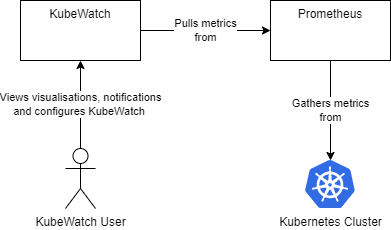
\includegraphics[height=5cm]{resources/System_context_diagram.png}
  \caption{System context diagram}
  \label{fig:system-context-diagram}
\end{figure}

\begin{figure}[H]
  \centering
  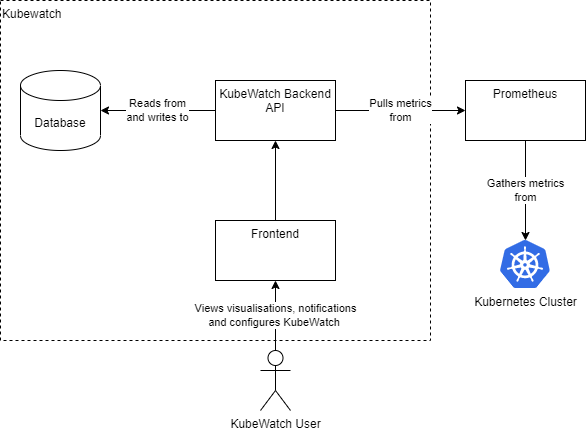
\includegraphics[height=8cm]{resources/Container_diagram.png}
  \caption{Container diagram}
  \label{fig:container-diagram}
\end{figure}

\begin{table}[H]
  \begin{tabular*}{\textwidth}{p{3.5cm} | p{9cm}}
    \textbf{Master:}
      & Each Kubernetes cluster contains at least one master node which runs the Kubernetes control plane. These control plane consists of an API server, scheduler, controller manager, etc. \bigskip \\
    \textbf{Worker/Node:}
      & Each cluster includes at least one worker node, this node runs containerized applications. Each worker node host \textit{Pods}. \bigskip \\
    \textbf{Pod:}
      & A pod is a component of the application workload. \\
  \end{tabular*}
  \caption{K8s elements explained}
  \label{tab:k8s-elements-explained}
\end{table}

\begin{figure}[H]
  \centering
  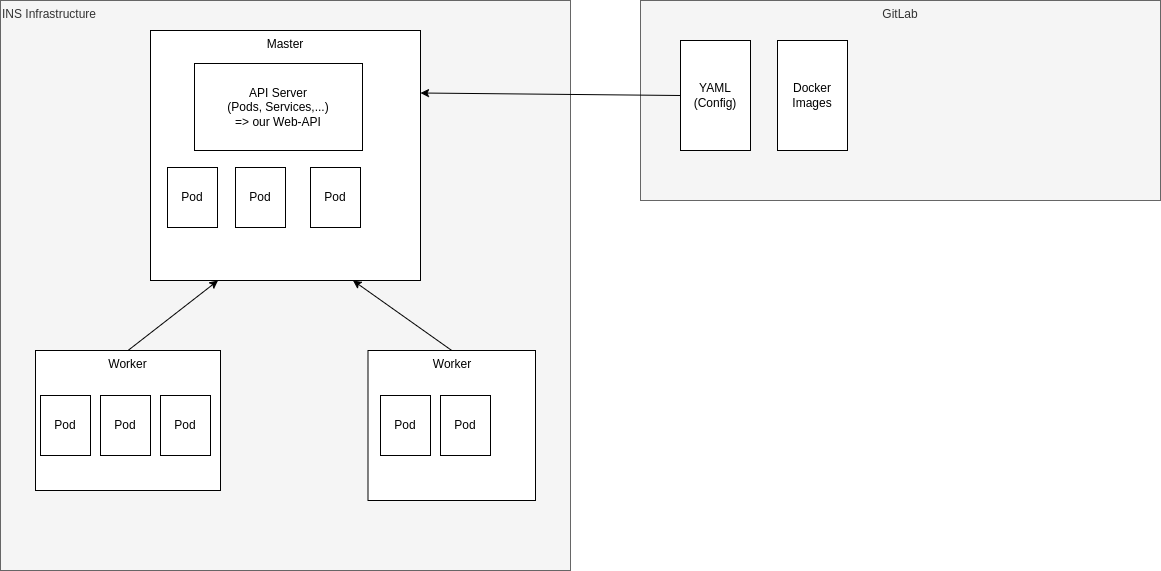
\includegraphics[height=7.3cm]{resources/architecture.png}
  \caption{KubeWatch CI/CD Pipeline architecture}
  \label{fig:architecture}
\end{figure}

\section{Web App}
\begin{figure}[H]
  \centering
  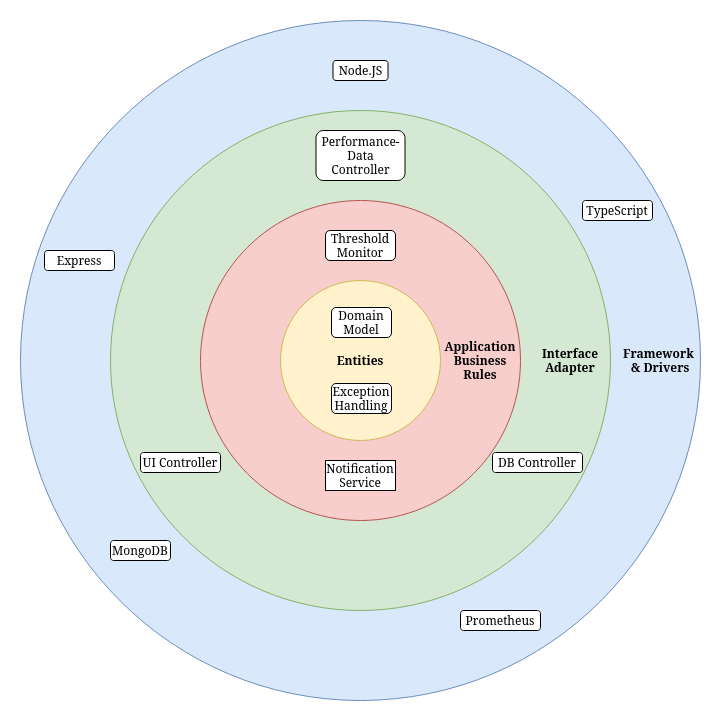
\includegraphics[height=14cm]{resources/clean_architecture.png}
  \caption{Web app clean architecture}
  \label{fig:web-app-architecture}
\end{figure}

\section{Wireframe}
The complete wireframe can be found as a PDF\footnote{\url{https://gitlab.ost.ch/SEProj/2022-FS/g03-kubewatch/kubewatch/-/blob/main/Documentation/appendix/wireframe_kubewatch.drawio.pdf}} and HTML page\footnote{\url{https://gitlab.ost.ch/SEProj/2022-FS/g03-kubewatch/kubewatch/-/blob/main/Documentation/appendix/wireframe_kubewatch.drawio.html}} in the appendix directory.
The HTML page is interactive.
